\documentclass[a4paper, 12pt]{article}
\usepackage[french]{babel}
\usepackage[T1]{fontenc}

%Lien hypertexte
\usepackage{hyperref}

%Paramétrage des marges
\usepackage[left=2.5cm,right=2.5cm,top=3cm,bottom=4cm]{geometry}

%Placement flottant des images
\usepackage{float}

%Inclure des images
\usepackage{graphicx}

%Légende
\usepackage{caption} 

%Paramétrage des pieds de page (et en-tête) + numérotation des pages
\usepackage{fancyhdr}
\pagestyle{fancy}
\usepackage{lastpage}
\renewcommand\headrulewidth{0pt}
\fancyhead[L]{}
\fancyhead[R]{}
\renewcommand\footrulewidth{0pt}
\fancyfoot[L]{Rapport de TIPE}
\fancyfoot[C]{}
\fancyfoot[R]{Page \textbf{\thepage} sur \textbf{\pageref{LastPage}}}

%Changement police des sections
\usepackage{titlesec}
\titleformat*{\section}{\Large\bfseries\sffamily}
\titleformat*{\subsection}{\large\bfseries\sffamily}
\titleformat*{\subsubsection}{\bfseries\sffamily}


\author{ \vspace{1cm} Arthur ALLAIN \& Fabien GOARDOU \& Thibaut RAOUL\\ 
		L2 CUPGE Technologies de l'Information\\
		École Supérieure d'Ingénieurs de Rennes\\ \vspace{1cm}
		Université de Rennes 1\\ 
		\texttt{\href{mailto:arthur.allain@etudiant.univ-rennes1.fr}{arthur.allain@etudiant.univ-rennes1.fr}}\\
		\texttt{\href{mailto:fabien.goardou@etudiant.univ-rennes1.fr}{fabien.goardou@etudiant.univ-rennes1.fr}}\\
		\texttt{\href{mailto:thibaut.raoul@etudiant.univ-rennes1.fr}{thibaut.raoul@etudiant.univ-rennes1.fr}}}
\title{{\textbf{Comment, par le biais d’une application, est-il possible de développer le e-commerce de proximité ?}\\(Rapport de TIPE)}}
\date{avril 2021}

\begin{document}
\maketitle
\begin{center}
	
\includegraphics[width=12cm]{fig/banniere_logos}
\end{center}
\thispagestyle{empty}
\newpage
\tableofcontents
\newpage
\listoffigures
\newpage
\section*{Remerciements}
\paragraph{}Nos plus sincères remerciements vont à tous les personnels et étudiants de l'Université de Rennes 1 qui nous ont permit de mener ce projet à bien.

\paragraph{}L'ensemble de l'équipe de TIPE remercie Johanne BÉZY-WENDLING pour ses conseils, son attention et ses encouragements durant toute la durée du projet.

\paragraph{}Nous remercions Olivier LAFOND pour sa motivation en tant que Responsable des CUPGE de l'ÉSIR dans le lancement et l'encadrement général des TIPE.

\paragraph{}Enfin, nous remercions la Direction des Systèmes d'Information de l'ISTIC pour la mise à disposition de la machine virtuelle et les précieuses réponses à nos questions. 

\newpage

\section{Introduction}

\paragraph{}L’année 2020, et la crise de la COVID, a bouleversé notre manière de vivre, d'interagir avec le monde extérieur et donc de consommer. Les périodes de confinement successives ont contraint les commerçants et les consommateurs à adapter, pour les uns, leur manière de vendre et, pour les autres, leur manière de consommer. Ces mutations ont eu lieu non seulement en France mais aussi partout autour du Globe.
\paragraph{}La création d’un site de commerce en ligne (dit e-commerce) est possible mais peu aisée. Son développement requiert des compétences pointues dans le domaine des nouvelles technologies et plus particulièrement dans le développement de sites internet et l'ingénierie logicielle. Nous pouvons alors nous demander comment, par le biais d’une application, il est possible de développer le e-commerce de proximité.
\paragraph{}Le but de ce projet est d’étudier la création d’un site internet et de permettre aux commerçants de proximité de vendre en ligne sur une marketplace (c’est-à-dire une place de marché). Un site internet abritant une marketplace a deux fonctions : permettre de vendre et permettre d’acheter.
\paragraph{}Ce projet est un projet ambitieux qui présente néanmoins des risques. Il est probable que nous rencontrions des difficultés dans le développement informatique. De plus, ce projet n’as pas pour but d’expliquer les différentes techniques de commerce ou les nombreux défis liés à la logistique. Enfin, notre solution n’aura pour objectif que de permettre le commerce à petite échelle.

\newpage
\section{État de l'Art}
\paragraph{}Avant de début la conception et la réalisation d'une solution informatique, il convient de faire l'état des solutions existantes et des technologies permettant d'en créer une.
\subsection{État du marché}
\subsubsection{La visite aux commerçants}

\paragraph{}Afin de comprendre au mieux les attentes des professionnels du commerce, nous avons été à la rencontre des commerçants. Notre objectif, lors de cette séance de rencontres, était de cerner au mieux leurs besoins et d’écouter leurs remarques sur les idées que nous avions.
\paragraph{}Nous avons été voir une épicerie Bio, une fleuriste et une boucherie/charcuterie. Parmi ces commerçants, seuls deux ont accepté de répondre à nos questions, la fleuriste ne pouvant pas répondre aux questions posées.
\paragraph{}La gérante de l’épicerie Bio s’est dite très intéressée car déjà en discussion avec un cabinet d’Audit parisien afin de mettre en place une marketplace pour leur magasin. Leur point de vue est que l’idée est intéressante uniquement si plusieurs commerçants d’un même secteur, d’une même commune par exemple, sont inscrits sur la plateforme. Ainsi, l’intérêt du site repose dans son adoption par les professionnels.
\paragraph{}La rencontre avec la boucherie-charcuterie a, quant à elle, été plus nuancée car les gérants de ce commerce nous ont répondu que leur modèle commercial était basé sur la vente de produits frais rares. Par exemple, une carcasse de bête achetée par le boucher est transformée dans la matinée et vendue par la suite dans la journée. Le temps entre la réception, la transformation et la vente de la marchandise n’est pas assez important pour référencer les produits en vente sur une plateforme. De plus, les bouchers de proximité ne travaillent pas à une échelle industrielle : les denrées achetées ne sont pas extensibles. Ainsi, ce boucher refusera une commande de vingt bavettes car il n’est pas capable de l’honorer. Ce type de commerce ne permet donc pas un déploiement sur internet car il s’agit de denrées fraîches et transformées rapidement. Ce n’est pas le cas pour de la marchandise sèche.

\subsubsection{Les objectifs}

\paragraph{}Les rencontres avec les commerçants nous ont permis d’étoffer notre projet. La solution proposée doit permettre aux commerçants de vendre leurs produits sur internet. De plus, celle-ci doit s’adapter aux contraintes de chaque commerce afin de faciliter l’adoption par le plus grand nombre de commerçants possible. Si un commerce n’est pas compatible avec le commerce en ligne, il peut, s’il le souhaite, être référencé sur le site internet afin d'apporter de la visibilité à son commerce. Cette solution permet de répandre l’utilisation du site internet parmi les commerçants d’une même commune : il est dans leur intérêt de gagner en visibilité en s’inscrivant sur le site internet.

\subsection{Les concurrents}
\subsubsection{Les solutions proposées}

\paragraph{}Durant les recherches effectuées lors du lancement du projet, deux types de solutions — parmi les concurrents potentiels — ont émergé. D’un côté, il est question d’une solution de marketplace, de l’autre, il est question de solution de création de site de e-commerce pour chaque commerçant client.
\paragraph{}La solution de marketplace (ou place de marché) est une solution qui consiste en une mise à disposition d’un espace, sur un site internet, “à des vendeurs indépendants moyennant une commission prélevée sur leurs ventes.” \cite{def_marketplace} Parmi les acteurs de ce secteur, qui mettent à disposition une marketplace sur internet dans le but de mettre en avant le commerce de proximité, notons la société Petitscommerces qui, selon eux, “valorise et accompagne les commerces de proximité indépendants sur le numérique” en éditant le site \url{www.petitscommerces.fr}. \cite{petitscommerces} Sur ce site, des commerces peuvent se référencer et référencer les produits qu’ils vendent. Cette société a l’avantage d’être bien implantée à Paris puisque plus de cent commerçants sont inscrits sur ce site dans la capitale française. En revanche, aucun commerçant breton n’est inscrit sur ce site. Le commerce référencé le plus proche de Rennes est un commerçant de La Baule.
\paragraph{}Une société concurrente de Petitscommerces est la start-up \textit{Ma Ville Mon Shopping}, devenue filiale de La Poste \cite{mavillemonshopping}. Cette société propose un site internet, du même nom, qui propose la mise à disposition d’une marketplace, c’est aussi une société de conseil avec des commerciaux parcourant les villes afin de faire la promotion de leur plateforme. Cette société comporte, elle, un catalogue fourni y compris dans le territoire breton. Les commerçants peuvent y référencer leurs produits et la société propose une solution de click-and-collect, de livraison en partenariat avec La Poste. La synergie entre la société de e-commerce et la société de transport est un point en faveur de la marketplace.
\paragraph{}La deuxième solution proposée par les sociétés est de créer un site de e-commerce pour chaque commerçant faisant appel à elles. La société \textit{Shopify} est une société canadienne, cotée à la bourse de New York (NYSE) et à la bourse de Toronto (TSX) \cite{shopify}, proposant de créer un site de e-commerce pour ses clients. Elle propose aussi de gérer la logistique et l’envoie des produits avec une offre de Dropshipping, ce qui permet au commerçant de se concentrer sur son activité de commerçant physique et non sur ses activités de e-commerce. Cette solution peut être adaptée pour les Denrées Non Périssables (abrégé DNP en vocabulaire commercial) mais en aucun cas un boulanger pourrait, par exemple, en faire l’usage.
\paragraph{}La deuxième société proposant, elle aussi, la création de e-commerce pour un commerçant unique, ou pour une agglomération, est la société \textit{Ma Boutique En Ville}. Cette société se concentre sur les commerçants de la région Auvergne-Rhône-Alpes d’où elle est originaire. Le site internet \cite{maboutiqueenville} de la société promet une création de marketplace pour les commerçants en une semaine. La rapidité de mise en place de la solution est donc un point crucial pour se démarquer dans la guerre des solutions de e-commerce.

\subsubsection{Une solution en adéquations avec les demandes}

\paragraph{}L'innovation proposée par les acteurs déjà présents sur le marché des sites de e-commerce local est de taille. Par conséquent, il revient à la solution proposée d’être ambitieuse afin de pouvoir espérer s’imposer auprès des commerçants ruraux et urbains de France.
\paragraph{}Afin de pouvoir toucher le plus de monde possible, la solution de la marketplace commune aux différents commerçants s’impose comme une solution viable et efficace. En effet, la visibilité d’un commerçant est ainsi assurée par la participation au commerce des autres commerçants d’un même secteur. De cette manière, plus le nombre de commerçants est important, plus le trafic sur le site est important ainsi l'adhésion de certains commerçants entraîne celle de leur confrères.
\paragraph{}Proposer une solution qui se démarque des concurrents passe par une offre étoffée de services autour de la marketplace : le but est, non seulement, de permettre au commerçant de vendre ses produits en ligne mais aussi de faciliter la gestion de son commerce. C’est pour cela que l’objectif est de proposer, en plus de la marketplace, une solution de gestion de stock pour faciliter la logistique de l’enseigne, qu’elle soit petite ou grande, qui peut parfois se révéler être un casse-tête. Les fonctionnalités de marketplace et de logistique rigoureusement combinées pourraient permettre une gestion plus simple de la comptabilité, et par dessous tout de la trésorerie, de l’entreprise.

\subsection{Les technologies disponibles}

\subsubsection{Les technologies pour le serveur}
\paragraph{}Le serveur est la partie de notre application qui gère toutes les informations. Le serveur doit tourner en permanence, autoriser ou non des personnes à se connecter, gérer les commandes. Le choix du langage serveur a été difficile, car nous avons ces différents langages possibles :

\begin{itemize}
	\item PHP : simple d’utilisation, peu sécurisé, lent, non typé
	\item Javascript : compliqué à prendre en main, grande diversité de bibliothèques, non typé
	\item Java : fiable, rapide, typé, orienté objet
\end{itemize}

\paragraph{}Un langage typé signifie que l’on doit expressément indiquer le type de nos données. Il permet de facilement utiliser la Programmation Orientée Objet (POO), afin de produire un code propre et avec un comportement fiable. 

\begin{figure}[H]
	\begin{center}
		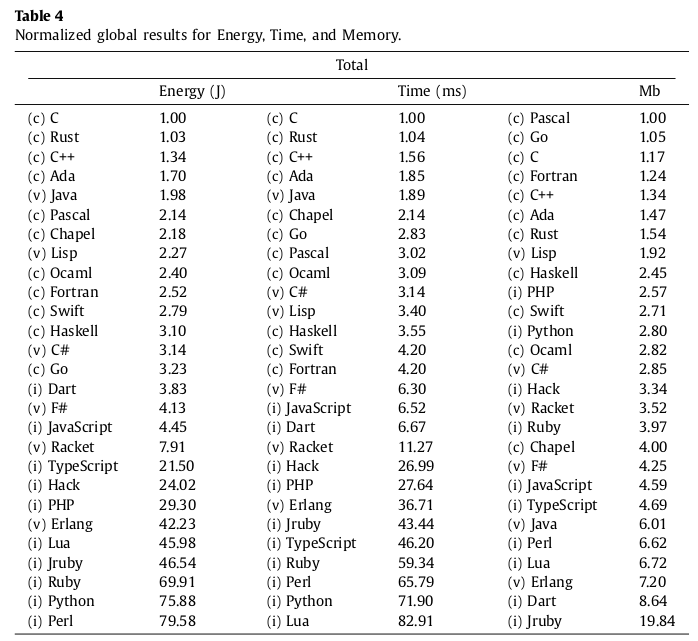
\includegraphics[width=10cm]{fig/tableLang}
		\caption{Normalized global results for Energy, Time, and Memory.\cite{pereira_ranking_2021}}
	\end{center}
\end{figure}

\paragraph{}Nous nous sommes donc tournés vers le langage Java qui possède ces deux caractéristiques. On peut voir en Figure 1 que ce n’est pas le plus rapide, car il est derrière le C et C++. Cependant, ce sont des langages beaucoup plus avancés et non accessibles pour un petit projet comme le nôtre, ce nécessitant pas de grandes optimisations.
\paragraph{}Afin de pouvoir sauvegarder nos données de façon permanente (catalogue d’un magasin, commandes passées...), nous avons choisis une base de données MySQL. Une base de données permet de sauvegarder et de récupérer rapidement des données persistantes (ne sont pas perdues si le programme s'éteint).  Le MySQL permet, comme avec le Java, de définir les types de données qui vont être sauvegardées. On assure avec cela que les données attendues sont fiables.

\paragraph{}Afin de gérer la liaison entre les clients et le serveur, une interface de programmation (API) est nécessaire. Nous avons fait le choix de faire appel à un framework qui a comme avantage d’être fourni avec toutes les fonctions de discussion avec le réseau. Ce framework nous permet de nous concentrer sur la liaison client-serveur qui est le cœur du problème.

\paragraph{}Afin de faciliter le déploiement de l’application, l’application serveur est lancée dans un container Docker. Cette technologie simule un environnement de travail indépendant de la machine sur laquelle elle est exécutée. Nous application serveur est donc exécutable sur n’importe quelle machine et ne nécessite aucune installation de dépendance. Cela facilite le travail du développeur, et de l’administrateur réseau lors du déploiement.

\paragraph{}L’hébergement du service est une étape importante dans le déploiement et ne doit pas être négligé. Afin d’être libre de nos mouvements sans avoir à payer quelque somme que ce soit, nous nous sommes tournés vers les machines virtuelles mises à disposition par l’ISTIC. Celles-ci sont fournies avec assez de mémoire vive (4Go) pour permettre à une API et un Base de Données de fonctionner en simultané. Cependant, une utilisation massive du site internet demanderait de dédier un budget considérable à son hébergement. Comme nous sommes dans un projet universitaire, une machine virtuelle suffira amplement.

\subsubsection{Les technologies pour le client}

\paragraph{}Afin de rendre notre application la plus accessible, nous avons décidé d’utiliser un site web pour le client. Ce site web sera la principale interface entre l’utilisateur et le serveur.
\paragraph{}Le monde du web est composé d’un nombre restreint de langages de programmation. Effectivement, une page web est principalement composée de :

\begin{itemize}
	\item HTML pour l’architecture
	\item CSS pour le rendu visuel
	\item Javascript pour les interactions utilisateur
\end{itemize}

\paragraph{}Certains Framework Javascript sont disponibles pour faciliter la programmation et avec un meilleur rendu visuel. Cependant, cela rajoute une couche d’abstraction à notre application. Plus précisément, cela veut dire qu’il y a moins de contrôle possible sur ce que l’on veut faire. Cela veut aussi dire que si on utilise qu’une petite partie de ce framework, il faut de toute manière que l’utilisateur télécharge tout le contenu. Nous avons donc choisis de ne pas utiliser de framework côté client, afin de garder une rapidité d’affichage de la page.
\paragraph{}Grâce à notre architecture serveur, il est possible de créer une application mobile et d’utiliser notre API accessible de n’importe où.

\subsection{Les contraintes}

\paragraph{}Un certain nombre de contraintes s’impose à nous. Elles sont légales ou bien pratiques et uniquement surmontables dans le cas d’un déploiement réel du projet.
\paragraph{Les contraintes légales}Premièrement, les contraintes s’imposant à notre projet peuvent être légales. Le commerce en ligne est très réglementé, comme toute forme de commerce. Du code de commerce (articles L441-1 et L441-2), ensemble de loi encadrant le commerce en France, il convient de mentionner que les conditions générales de ventes sont obligatoires dans le cas de la création d’un site de e-commerce car “Toute personne exerçant des activités de production, de distribution ou de services qui établit des conditions générales de vente est tenue de les communiquer à tout acheteur qui en fait la demande pour une activité professionnelle.”\cite{code_commerce_1} Notre site, dans le cas d’une commercialisation des services, devrait en bénéficier. Les conditions générales de ventes servent de socle à la négociation commerciale.\cite{code_commerce_1} Elles mentionnent les parties qui participent à l’échange commercial et les limites du lien qui les uni. Cette liste de clauses encadrant le commerce d’une entreprise est dans la majorité des cas rédigée par un avocat afin de protéger l’entreprise émettrice et de s’assurer de la légalité des clauses qu’elle y inscrit.
\paragraph{}Les conditions générales d’utilisation et les mentions légales décrivent de la même manière le lien entre le consommateur et le fournisseur du service. Elles sont encadrées par le Code de la Consommation et comportent les informations légales identifiant la société productrice du service. \cite{code_consommation} Dans le cas d’un site internet, l’éditeur du site internet doit être mentionné, tout comme l’hébergeur de celui-ci. Elles encadrent les services mis à disposition du consommateur. Les conditions générales d’utilisation sont, comme les conditions générales de ventes, rédigées le plus souvent par un avocat afin de protéger le consommateur et le fournisseur du service et de s’assurer de la conformité du document.
\paragraph{}Les contraintes légales ne s’appliquent pas au niveau Français uniquement. Le règlement européen sur la protection des données personnelles (abrégé RGPD) encadre le stockage et l’utilisation des données personnelles recueillies par une société. Cet ensemble de quatre-vingt-dix-neuf articles de lois mentionne notamment que tout utilisateur dispose d’un droit de regard sur les données qu’une entreprise dispose sur lui. Il s’applique pour toute entreprise commerçant sur le sol européen.  Par exemple, un site internet édité aux États-Unis d’Amérique et hébergé sur le sol américain se doit de respecter le RGPD dans la mesure où un individu utilise le service en Europe (Article 3) \cite{rgpd} . L’article 15 précise que l’utilisateur dispose d’un droit d’accès sur les informations dont le site dispose sur celui-ci. L’article 7 précise que le consentement de l’utilisateur est requis pour tout recueillement de données sur celui-ci. Le respect de ce document est important et nous oblige à prévoir un moyen pour l’utilisateur d’accéder aux informations dont le site dispose sur sa personne. Nous devons, aussi, absolument recueillir le consentement de l’individu avant de stocker toute donnée.
\paragraph{Les contraintes techniques}De surcroît, certaines contraintes pratiques sont réservées aux sociétés déployant réellement leur produit. Ces contraintes nécessitent la signature de contrats avec des sociétés tierces.
\paragraph{}Par exemple, le paiement en ligne requiert la contraction d’un accord avec une banque, ou avec une société auxiliaire assurant la liaison banque-société utilisatrice, afin de permettre à l’utilisateur de payer directement sur le site internet. Notons que la conservation des données bancaires est limitée et réglementée par la CNIL. \cite{payonline} Ces contrats et les intégrations des services des prestataires ne sont pas simulables à l’échelle visée et la signature d’un contrat n’est pas envisageable au vu de la portée universitaire d’un tel projet.
\paragraph{}La mise en place de la livraison n’est possible que si le commerçant l’assure. En effet, il n’est pas envisageable de signer un contrat avec une société de livraison, bien qu’il existe des sociétés prenant en charge les denrées alimentaires périssables, pour les mêmes raisons que cité précédemment. Notons en revanche que la livraison n’est pas forcément liée à une empreinte carbone négative puisque des livraisons sur courtes distances sont possibles à vélo, ce qui réduit considérablement l'empreinte.
\paragraph{}L’envergure de ce projet implique que certaines de ses contraintes seront évitées afin de se concentrer sur la production. Dans la partie encadrant légalement les activités, seul le RGPD sera mentionné sur le site internet car des données utilisateur doivent être stockées pour la création d’un compte. Les moyens de paiement et de livraison ne seront, eux, pas disponibles car il n’est techniquement pas possible de les mettre en place.

\newpage
\section{Conception}
\subsection{La méthodologie de travail}
\subsubsection{La répartition du travail}
\paragraph{}Afin de mener à bien le projet, nous avons décidé de répartir les tâches de manière assez uniforme : chaque membre de l’équipe a été mis en charge d’une partie distincte. Le groupe étant composé de trois membres, le travail de production a été divisé en trois parties : le développement du serveur (Back-end), le développement de la liaison entre le client et le serveur (API) et le développement du client (Front-end).
\paragraph{}Les différentes tâches à effectuer ont été inscrites dans un scrum-board ce qui a permis de suivre l’avancement de chaque personne. Cette méthode a aussi permis un suivi plus simple des activités par l’encadrant.
\paragraph{}Lorsqu’une partie du développement fut fini, la personne chargée de celui-ci fut réorientée vers les parties nécessitant encore du développement actif. Par exemple, le développement du serveur achevé, le développeur de celui-ci s’est réorienté vers le développement du client web.
Cette répartition a permis un avancement habile et souple pour mener à bien le projet.
\subsubsection{Le processus de conception}
\paragraph{}Le processus de conception, c’est-à-dire la méthode utilisée pour construire, est très important dans un projet de cette envergure car il permet d’optimiser le temps accordé à une partie.
\paragraph{}Le développement dirigé par les tests (appelé plus couramment TDD) consiste en l’écriture des tests avant le développement du code source. Cette technique, enseignée et utilisée à grande échelle, permet de ne pas complexifier le développement en ajoutant des temps de débuggage en plus du développement. Le code développé passe forcément les tests car il a été écrit en fonction de ceux-ci.

\begin{figure}[H]
	\begin{center}
		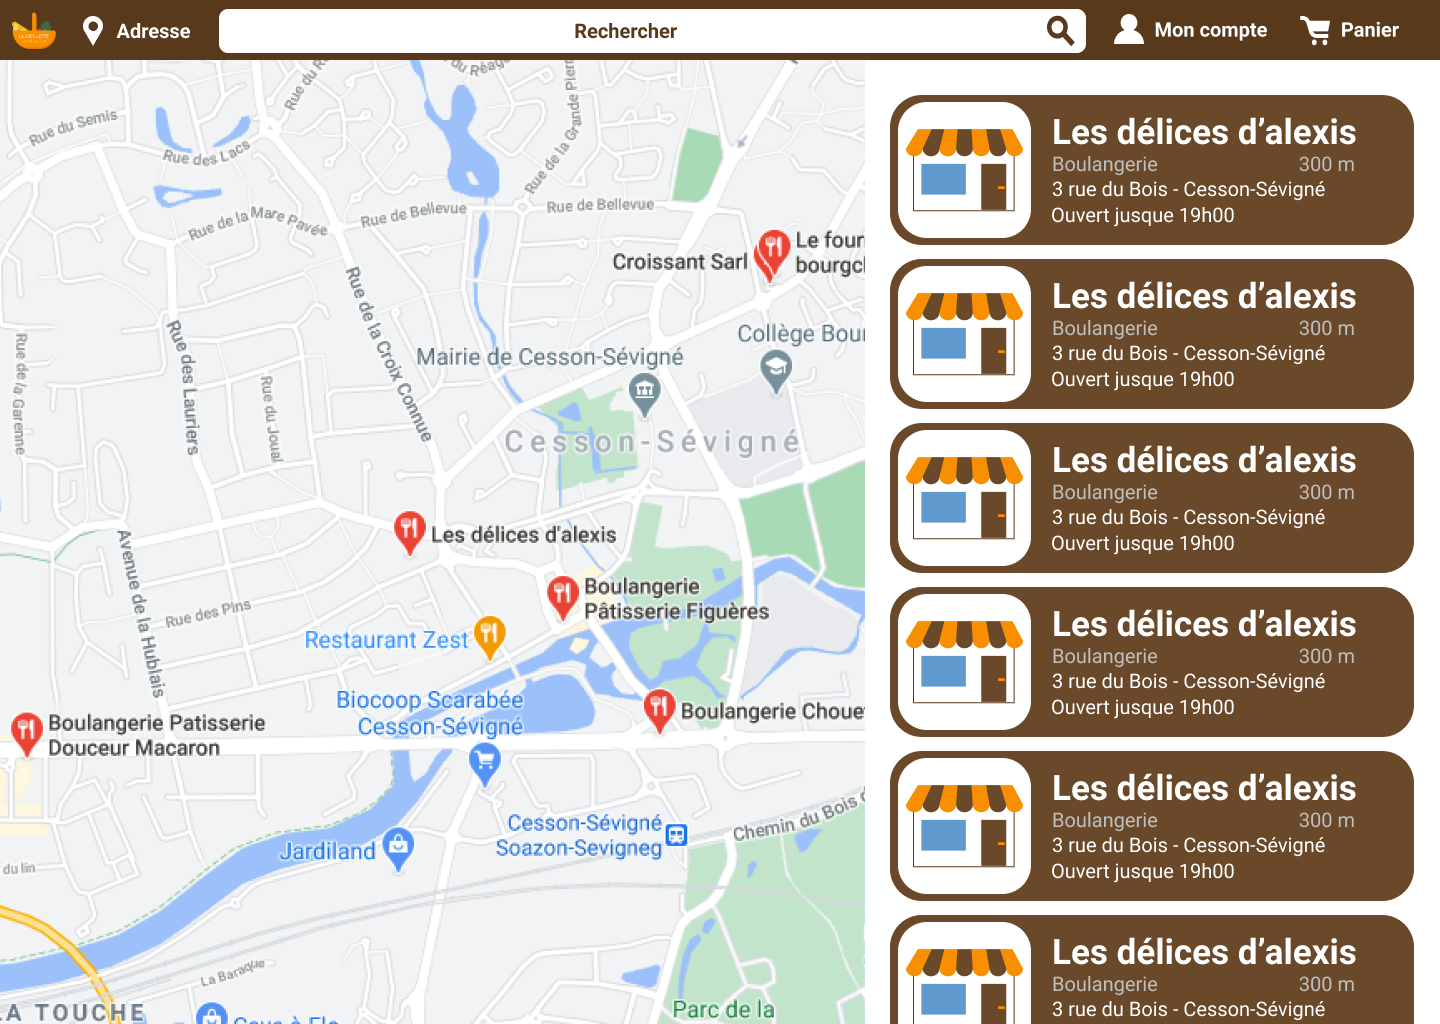
\includegraphics[width=10cm]{fig/maquette.png}
		\caption{Maquette de construction de l'interface graphique du site internet}
	\end{center}
\end{figure}

\paragraph{}L’interface graphique nécessite la conception d’une maquette graphique au préalable afin que le développeur en charge du développement de l’interface graphique sache vers quel design s’orienter sans perdre du temps à tergiverser. Cette maquette (Figure n°2) a, de toute évidence évolué entre sa première version et la version actuelle du site internet, cependant il est indéniable qu’elle a permis de gagner beaucoup de temps dans les grandes parties graphiques de l’interface.

\subsection{La réalisation}
\subsubsection{Le back-end}

\paragraph{}Le serveur est la section de la solution qui gère l’inscription et la lecture dans un registre général : la base de données.
\paragraph{}Afin de pouvoir mettre en vente et acheter des produits, nous avons modélisé sous forme d’un objet, en java, les produits, les magasins, les utilisateurs et tous les éléments nécessaires à la vente à distance. Le processus de modélisation, la fabrication de l'architecture logicielle, est une étape cruciale car elle définit l’agilité avec laquelle le développeur va pouvoir accéder aux différents éléments du programme.
\paragraph{}L’architecture logicielle que nous avons fabriquée est le schéma de la communion entre la base de données (créée en MySQL) et le programme (écrit en Java) qui lit et écrit sur la base de données. Notre logiciel en est le résultat. Chaque action de l’utilisateur (connexion, mise en ligne d’un article, mise au panier d’un autre, etc.) est enregistrée dans la base de données. Le programme reflète ce que la base de données a enregistré.

\begin{figure}[H]
	\begin{center}
		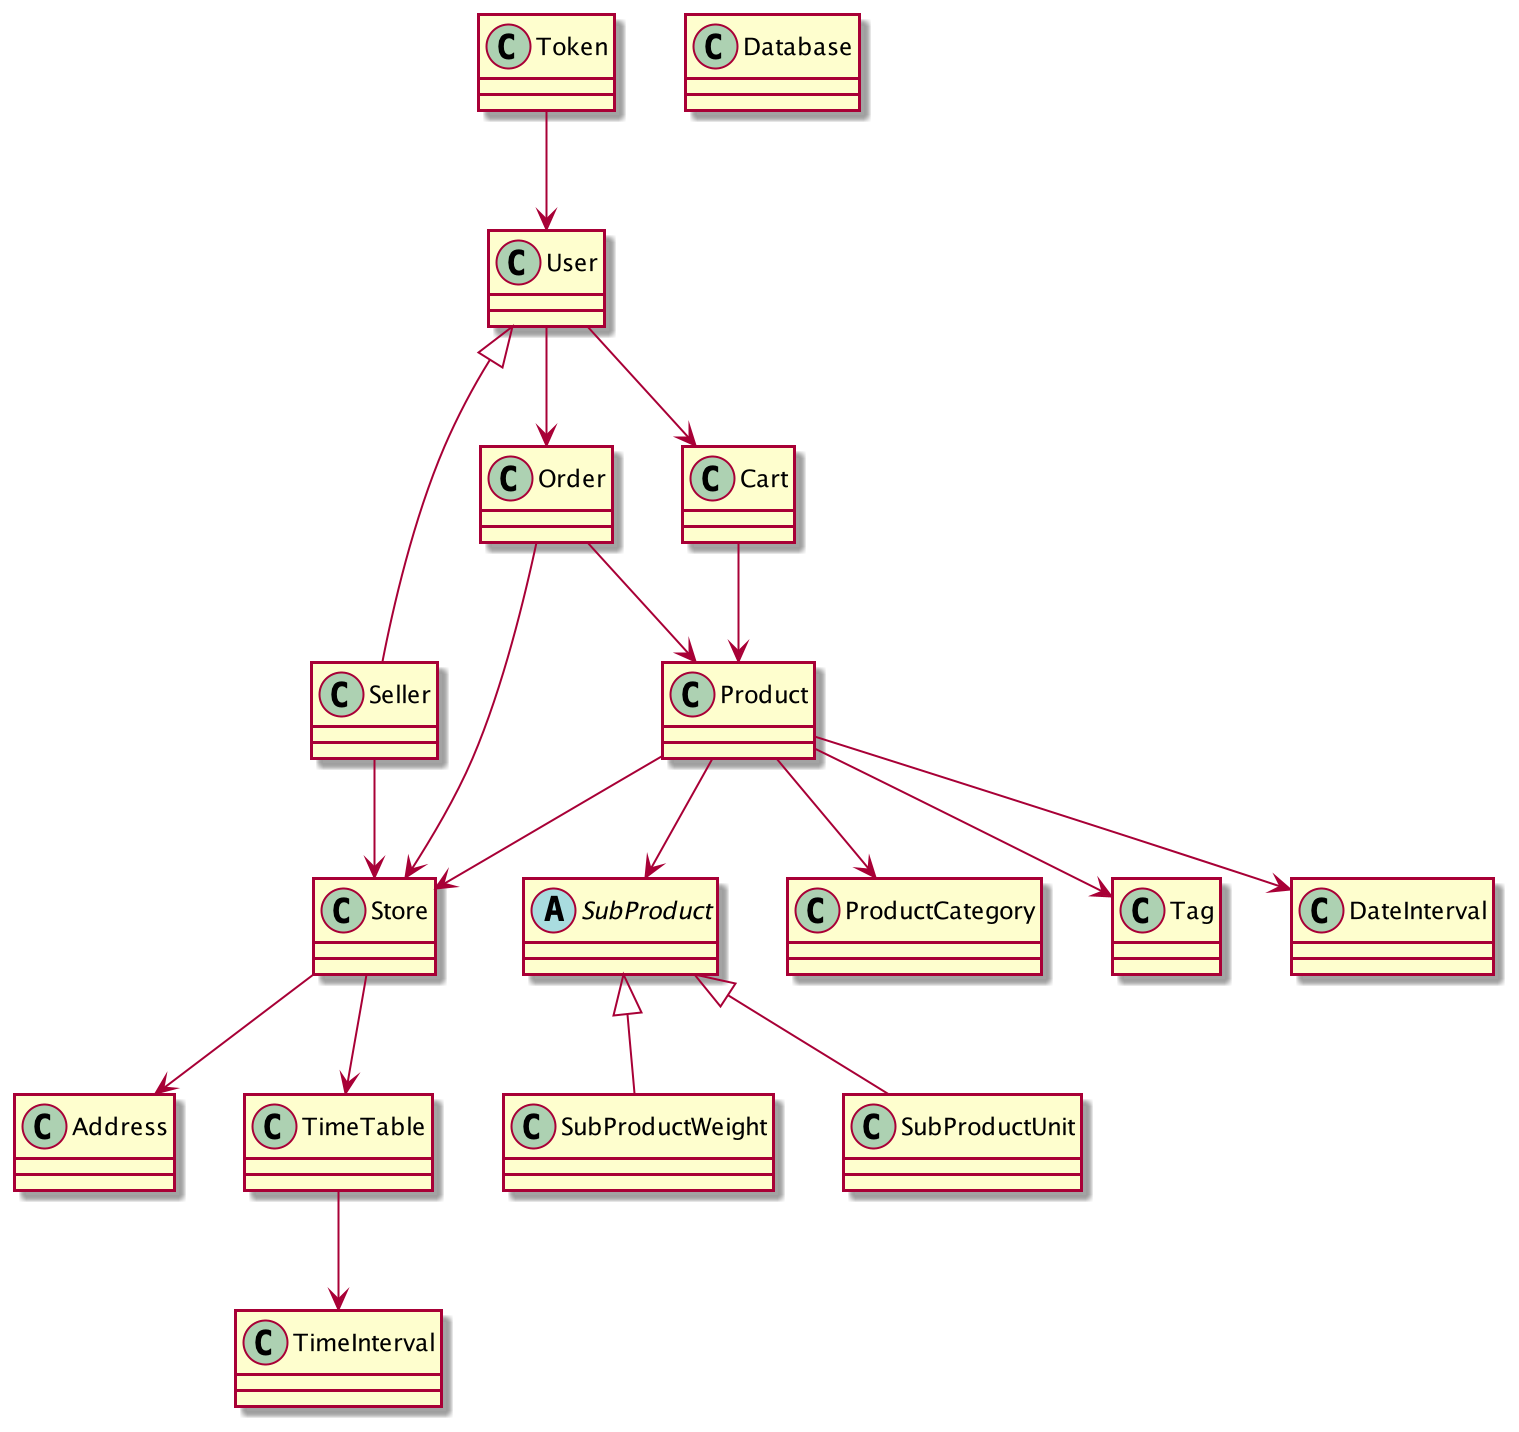
\includegraphics[width=10cm]{fig/uml-simplified.png}
		\caption{Diagramme UML de l'architecture du moteur serveur du produit}
	\end{center}
\end{figure}

\paragraph{}Comme mentionné sur la Figure n°3, de l’adresse au sous-produit tout concept utilisé dans le programme est représenté par des variables.  Cette modélisation est présente dans la base de données MySQL et dans la mémoire vive de l’ordinateur exécutant le logiciel serveur (que l’on appelle, pour simplifier, serveur). L’interface avec l’interface de programmation (l’API) s’opère grâce à des méthodes de mutations (plus couramment appelées Getters and Setters).

\subsubsection{L'API}

\paragraph{}L’interface de programmation (API) fait la liaison entre la partie cachée de la solution (le serveur) et sa partie visible (le client). L’utilisation de l’API ne nécessite pas de savoir comment fonctionne le serveur, la documentation fournie par le développeur de celle-ci permet de connaître quel point d’entrée est à utiliser pour obtenir l’information recherchée. L’utilisation de l’API s’organise à travers des requêtes et des réponses, sa programmation se concentre sur les mêmes aspects.
\paragraph{}Grâce aux méthodes de mutations mises à disposition précédemment, l’interface de programmation gère les accès aux données et vérifie si l’utilisateur qui requiert une information a le droit d’y avoir accès. Quand une requête est envoyée à l’API, celle-ci vérifie la qualité de l’utilisateur puis demande au programme les données recherchées. Une modification est faite dans le programme et dans la base de données s’il est nécessaire d’en faire. Une réponse est ensuite remise à l’utilisateur qui en a fait la demande.
\paragraph{}Grâce au Framework Spring, le développement de cette interface de programmation est amplement simplifié. Le développeur s’est concentré sur les suites d’opérations à faire mais le service de discussion avec le client est, pour sa part, déjà prêt à l’emploi. Le démarrage du programme entraîne le démarrage de la couche fournie par Spring et permet la discussion sur le réseau entre des ordinateurs.
\noindent Une API fonctionnelle permet au client de fonctionner correctement.

\subsubsection{Le front-end}

\paragraph{}Le client est roi. C’est une maxime que nous pourrions utiliser pour décrire la construction de l’interface graphique que nous avons construite pour l’utilisateur. L’accent a été mis sur la simplicité et la facilité d’utilisation de la solution pour que le plus large public possible puisse y accéder et sans servir sans se casser la tête.
\paragraph{}La conception en application web du client internet permet au site internet de s’adapter à toute taille d’écran sans nécessiter le rafraichissement de la page internet : que le site soit chargé sur un smartphone, une tablette ou un ordinateur, l’affichage est toujours parfait. Cette solution permet à l’utilisateur d’avoir l’impression d’utiliser un logiciel fait spécifiquement pour son moyen d’accès alors qu’il est fait pour tous les moyens à la fois.
\paragraph{}La fabrication du client Front-end consiste en l’ajout de composants graphiques et en la soumission de requêtes, avec ces composants, au serveur et à la réception des réponses (à travers l’API). C’est une tâche longue car la fabrication de l’interface est un éternel processus d’essai-tests pour savoir où placer un module et comment l’habiller.
\paragraph{}L’agrégation et la mise en œuvre de ces méthodes de travail nous ont permis de fabriquer une interface permettant de mettre en vente et d’acheter des produits en ligne.

\subsection{Les résultats}
\subsubsection{Notre solution de e-commerce de proximité : La Cueillette}

\paragraph{}Après avoir étudié la conception d’une solution pour permettre aux utilisateurs d’acheter et de vendre des produits en ligne, après avoir suivi les méthodes de travail et fabriqué le site internet que nous avions inventé, nous sommes en mesure de proposer une solution.
\paragraph{}[PAGE D’ACCUEIL (À venir bientôt...)]
\paragraph{}Nous pouvons observer, sur la Figure [INSÉRER LE NUMÉRO], la page de garde du site internet \href{https://www.lacueillette.ml}{www.lacueillette.ml}. Cette page invite l’utilisateur à rechercher un produit sur le site internet ou à se connecter afin d’accéder à son panier, ses commandes ou ses informations.
\paragraph{}[PAGE D’UN PRODUIT (À venir bientôt...)]
\paragraph{}La recherche d’un produit sur le site internet mène à une liste de produits se rapprochant, par les mots-clé de leur titre, du mot ou de la suite de mots entrés dans la barre de recherche. L’utilisateur peut alors choisir le produit qui l’intéresse, il arrive alors sur la fiche produit (Figure [INSÉRER LE NUMÉRO]). Par la suite, si le produit correspond à ses besoins ou à ses envies, le client peut ajouter ce produit dans son panier (en modifiant la quantité qu’il désire, si nécessaire). Il peut, par la suite, se rendre dans son panier pour consulter l’intégralité de ses commandes en devenir.
\paragraph{}[PAGE D’UN AJOUT DE PRODUIT (À venir bientôt...)]
\paragraph{}Un utilisateur commerçant peut demander l’ouverture d’un magasin (réplique de son magasin physique) sur la page de son compte utilisateur. Il peut, par la suite, ajouter des produits à son magasin.  La Figure n°[INSÉRER LE NUMÉRO] fait état de la fiche de renseignement qu’il faut remplir pour chaque produit. Notons par exemple, qu’il est nécessaire d’entrer un nom, un prix et un taux de TVA (Taxe sur la Valeur Ajoutée) pour chaque produit. Le commerçant peut, par la suite, ajouter ou modifier la fiche de son produit. Dès l’enregistrement de son formulaire, le produit est en ligne sur le site La Cueillette.

\subsubsection{Ce que l'on pourrait ajouter}

\paragraph{}Bien que l’énergie investie dans ce projet soit immensément importante, il n’a pas été possible de développer une solution complète. Nous pourrions alors ajouter de nouvelles fonctionnalités permettant de faciliter la vie du commerçant dans la gestion comptable et logistique de son commerce. L’agrégation de toutes les factures générées, la génération d’un bilan comptable, l’intégration aux caisses enregistreuses sont des pistes d’amélioration pouvant être envisagées.
\paragraph{}Nous pourrions aussi nous poser la question du déploiement à l’étranger et notamment en Europe où les mêmes problématiques de domination du marché par des géants américains posent les mêmes questions que sur le territoire Français. Ces améliorations commerciales sont envisageables et absolument réalisables à la vue de la souplesse de la solution informatique créée.


\newpage
\section{Conclusion}

\paragraph{}Au cours de ce TIPE, nous avions pour objectif d’étudier comment, par le biais d’une application, il est possible de développer le e-commerce de proximité. Nous avons donc trouvé plusieurs acteurs du commerce en ligne faisant la promotion de leurs services pour développer le secteur visé. Nous avons déterminé leur points positifs et négatifs, nous avons été à la rencontre des commerçants de nos villes, afin de déterminer quelle solution serait la meilleure pour développer le commerce en ligne de proximité.
\paragraph{}L’objectif qui était le nôtre n’était en aucun cas de construire en moins de six mois une solution ayant pour objectif de détrôner les leaders du commerce en ligne, nous avions pour objectif de découvrir et d’étudier la création d’un site internet de vente en ligne et de permettre la mise en ligne de produits ainsi que la consultation de ceux-ci.
\paragraph{}Pour arriver à nos fins, nous avons dans un premier temps étudier les méthodes de conception et de création de solutions informatiques permettant la discussion entre un client et un serveur. Nous avons ensuite créé l’architecture d’une solution permettant de répondre aux objectifs que nous nous étions fixés.
\paragraph{}Pour réaliser les tâches de production, nous avons décidé de répartir le travail en trois blocs pour que chaque membre puisse s'instruire et développer sa section à son rythme. Chaque section pouvant être améliorée, nous l’avons fait dans un processus d’amélioration continue concerté entre les membres de l’équipe projet.
\paragraph{}La solution proposée est fonctionnelle pour un nombre limité de fonctionnalités. Il est possible d'effectuer des opérations simples comme la mise en ligne d’un produit et l’ajout au panier de celui-ci. Il serait possible de dépasser ces limites si le projet devenait une réalité commerciale (ou même associative).
\paragraph{}D’autres améliorations seraient possibles, d’un point de vue graphique notamment, qui est un domaine requièrent un nombre incalculable de capacité pour construire une interface graphique fluide et facile à utiliser. Nous pourrions, par la suite, étudier la possibilité d’un lancement commercial dans l’Europe et à travers le monde.


\newpage
\section{Bibliographie}
\bibliographystyle{IEEEtran}
\bibliography{bibli}

\newpage
\section*{Annexes}
\subsection*{Diagramme UML complet du moteur du serveur}

\begin{figure}[H]
	\begin{center}
		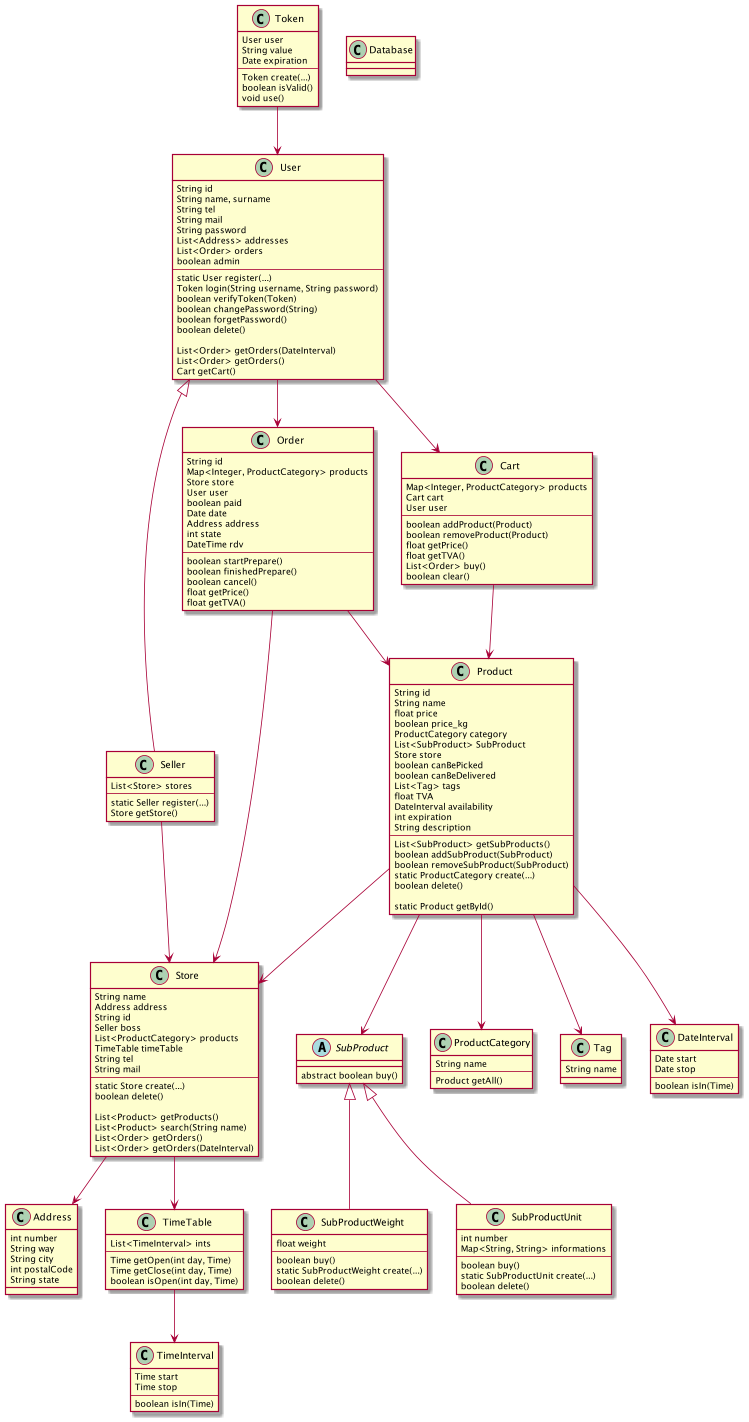
\includegraphics[width=10cm]{fig/uml-all.png}
		\caption*{Diagramme UML complet de l'architecture du moteur serveur du produit avec les attributs et les méthodes de chaque classe}
	\end{center}
\end{figure}

\end{document}